\documentclass{article}

\usepackage{booktabs}
\usepackage{tabularx}
\usepackage{hyperref}
\usepackage{graphicx}
\usepackage{pdflscape}


\hypersetup{
    colorlinks=true,       % false: boxed links; true: colored links
    linkcolor=red,          % color of internal links (change box color with linkbordercolor)
    citecolor=green,        % color of links to bibliography
    filecolor=magenta,      % color of file links
    urlcolor=cyan           % color of external links
}

\title{Hazard Analysis \\\progname Mission Control Terminal MC}

\author{Team 12, Autonomous Satellite Operations Scheduler\\ Diamond Ahuja \\ Rishi Vaya \\ Buu Ha \\ Umang Rajkarnikar \\ Dhruv Cheemakurti}

\date{\today}


\begin{document}

\maketitle

~\newpage

\pagenumbering{roman}

\begin{table}[hp]
\caption{Revision History} \label{TblRevisionHistory}
\begin{tabularx}{\textwidth}{llX}
\toprule
\textbf{Date} & \textbf{Developer(s)} & \textbf{Change}\\
\midrule
October 20, 2023 & Q.H, R.V, D.A, D.C, U.R & Completed HA documentation\\
\bottomrule
\end{tabularx}
\end{table}

~\newpage

\tableofcontents

~\newpage

\pagenumbering{arabic}


\section{Introduction}
The primary objective of our project MCT (Mission Control Terminal) is to provide satellite operators with a platform to automatically schedule and send commands to satellites as they pass overhead. In addition, the system will keep logs of all commands sent, responses, with concurrent access available. This is a hazard analysis document for the MCT capstone project.

\section{Scope and Purpose of Hazard Analysis}
Hazard Definition - Hazards can be defined as any situation within an application that can potentially lead to an unwanted or undesirable outcome which can include system failures, data loss, harm to users or any other consequences. These hazards can occur due to many factors such as design flaws, communication flaws, equipment failures and programming errors. 

The purpose of this document is to find cases of hazards that may be encountered in the project and find potential methods to mitigate those hazards.

\section{System Components}
\begin{itemize}
    \item Command Scheduling: 
Operators need to be able to schedule commands for engineering and NEUDOSE satellites. They should be able to work concurrently with other users

\item Orbital Prediction:
Operators need to be able to calculate and predict satellite overpasses and satellite illumination cycles.
 \item User Authentication and Authorization: 
Users must be able to log in, with a special admin user which controls access to satellite usage.


\item Logging:
Users must be able to retrieve a log of commands sent, and responses from the application.

\end{itemize}

\section{System Boundaries}
\begin{itemize}
    \item Satellite Hardware and Control Systems:
The application will not directly interface with the satellite’s hardware, it will send commands to the ground station for transmission.

\item Ground Station Infrastructure:
The application will not manage or control the ground station equipment.

\end{itemize}

\section{Critical Assumptions}

\begin{itemize}
\item The linux server hosting the web application shall not be suspended or paused.
\item The operator and system administrators using the application shall not misuse it or intentionally use it in an unintended way.
\item Operators and system administrators are well-informed of security best practices, such that they are aware of attacks like phishing attacks.
\item The authentication token provided by the OpenID Connect Protocol is cryptographically secure.
\item The commands are verified by the operators before they are scheduled.
\end{itemize}

\begin{landscape}
    \begin{figure}[p]
    \section{Failure Mode and Effect Analysis}
        \centering
        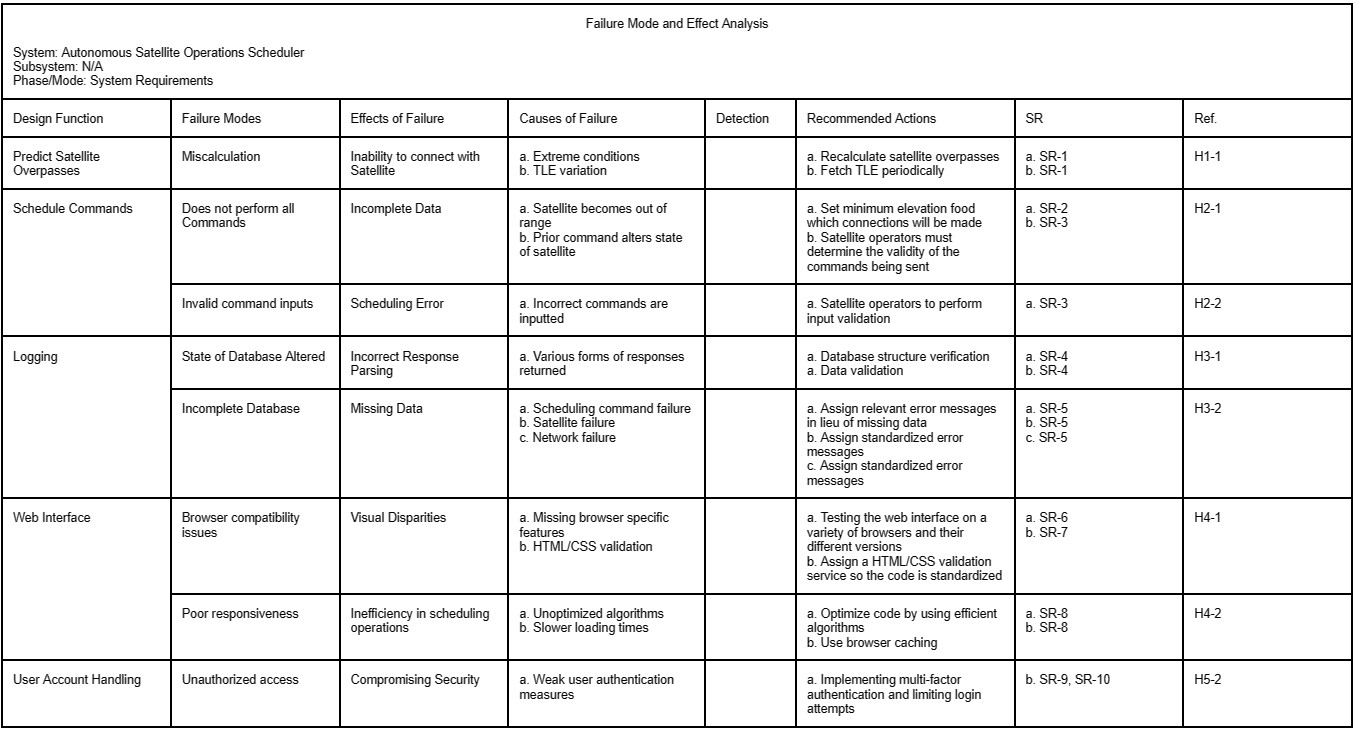
\includegraphics[width=1.16\linewidth]{FMEA.jpg}
        \caption{FMEA process}
        \label{fig:fmea_landscape}
    \end{figure}
\end{landscape}

\section{Safety and Security Requirements}

\subsection*{SR-1:}
The application shall periodically fetch TLE and calculate satellite overpasses to ensure the most recent data is being used to predict satellite overpasses. \\ \\
\textbf{Rationale:} An issue with calculating satellite overpasses is the variation in TLE and other conditions. Periodically retrieving and recalculating this piece of information will ensure a more accurate prediction of overpasses.  \\ \\
\textbf{Associated Hazards:}  H-1a, H-1b


\subsection*{SR-2:}
The application shall use a minimum elevation as a point of reference to evaluate whether a connection to the satellite can be made. \\ \\
\textbf{Rationale:} In the case that a satellite is below the minimum elevation required to make a connection, the scheduled commands may not work and as a result, produce incomplete data. By having a minimum point of reference, the system can assess if a satellite is out of range. \\ \\
\textbf{Associated Hazards:}  H-2a

\subsection*{SR-3:}
Operators shall be informed of errors that occur during the scheduling of commands, however, it is the operator’s responsibility to ensure the validity of the commands. \\ \\
\textbf{Rationale:} Since the application allows operators to send and schedule commands to the satellite, it is possible that an incorrect command is sent.  In this case, it would be helpful to highlight the errors found in the operator’s input data.  \\ \\
\textbf{Associated Hazards:}  H-2b, H-3a

\subsection*{SR-4:}
The system shall have a backup and recovery mechanism which is capable of restoring the database to its most recent correct state in the event of unexpected data failures. \\ \\
\textbf{Rationale:} A situation may occur where the database enters into an unknown or corrupt state. The presence of a backup and recovery mechanism ensures that the information in the database is still accessible by rolling back to the most recent correct state.  \\ \\
\textbf{Associated Hazards:}  H3-1a, H3-1b

\subsection*{SR-5}
In the event of a system, network, or satellite failure, all missing data fields shall be labelled with an appropriate error message as part of the data validation process. These error messages shall adhere to a standardized format. \\ \\
\textbf{Rationale} There may be cases where a scheduled command produces responses with missing data attributes. By identifying the incomplete data using standardized error messages, it provides a consistent data state across all validation processes. \\ \\
\textbf{Associated Hazards:} H3-2a, H3-2b, H3-2c

\subsection*{SR-6}
Cross-browser testing across a range of browsers shall be performed to ensure the application functions consistently. \\ \\
\textbf{Rationale} Due to slight variations in browsers such as Safari, Chrome, and Firefox, it is important to assess the performance of the application across all user-intended environments. \\ \\
\textbf{Associated Hazards:} H4-1a

\subsection*{SR-7}
The code base shall have HTML and CSS checks to ensure compatibility across different devices and browsers. \\ \\
\textbf{Rationale} Incorporating the above checks can identify errors in the code base as well as possibly improve the application’s user interface. \\ \\
\textbf{Associated Hazards:} H4-1b

\subsection*{SR-8}
All components which are required for scheduling operations shall be evaluated on their efficiency, where each component must complete within a minimum time frame. \\ \\
\textbf{Rationale} By having a pipeline to test parts of the duration of a code, it can prevent situations where there may exist an inefficiency in scheduling operations. \\ \\
\textbf{Associated Hazards:} H4-2a

\subsection*{SR-9}
The application shall not authenticate a user who has attempted to login with the same credentials ten times, consecutively. The application shall have a timeout period of five minutes before the user can authenticate themselves. \\ \\
\textbf{Rationale} By having a timeout period for a set number of unsuccessful authentication attempts, it protects user accounts from unauthorized access and improves security. \\ \\
\textbf{Associated Hazards:} H5-1a

\subsection*{SR-10}
The application shall support multi-factor authentication such that a user must verify their identity through their registered email account. \\ \\
\textbf{Rationale} Having multi-factor authentication provides an additional layer of security to the application, ensuring that unauthorized users are prohibited from accessing sensitive user and system data. \\ \\
\textbf{Associated Hazards:} H5-1a

\section{Roadmap}

The hazard analysis introduced a number of new safety and security requirements for the project. The team will ensure that most of the requirements are implemented by the time of the first demonstration in February, 2024. The primary focus will be on implementing all requirements except SR-4. The team believes that a secure database will already be used in the project and hence there is no immediate need for a backup. However, it was decided that this could be implemented in the future of the application.  

\end{document}